% ------------------------------------------------------------- 
% Arquivo :  relatório modelo                                        
% ------------------------------------------------------------- 

\documentclass[brazilian,12pt,a4paper,final]{article}
% tamanhos de fontes: 10pt, 11pt ou 12pt
% opções de estilo (padrões): article, report, book, slide, letter (artigo, relatorio, livro, apresentação de slides, carta)
\usepackage[brazil]{babel}     % ifenização
%\usepackage{t1enc}            % reconhecimento dos acentos inseridos com o teclado
\usepackage[utf8]{inputenc}    %  reconhecimento dos caracteres com codificação UTF8, acentuação.
\usepackage{graphicx}          % figuras em formato eps 
%\usepackage[pdftex]{graphicx} % para produzir PDF diretamente
%\usepackage{color}             % fontes soloridas
%%% fim do cabecalho %%%

\pagestyle{empty}
\title{Euler X Euler-Cromer}
\author{Aluno: Átila Leites Romero \\ Matrícula: 144679 \\ IF-UFRGS}

\begin{document}
\maketitle

\section*{Questão 3} 
Quando $k=1$ e $m=1$, o período é $\tau=2\pi$. 

Com $x(0)=1$ e $v(0)=1$, foram usados $\Delta t$ com os valores 
$0.06$, $0.24$, $0.42$, e $0.60$.

O programa, que recebe os parâmetros k,m,x,v,t0,tf,dt1,dt2,dt3,...
foi executado com 
\begin{verbatim}
./quest3.py 1 1 1 0 0 25.1328 0.06 0.24 0.42 0.60
\end{verbatim}
O gráfico gerado com o algorimo de Euler foi:

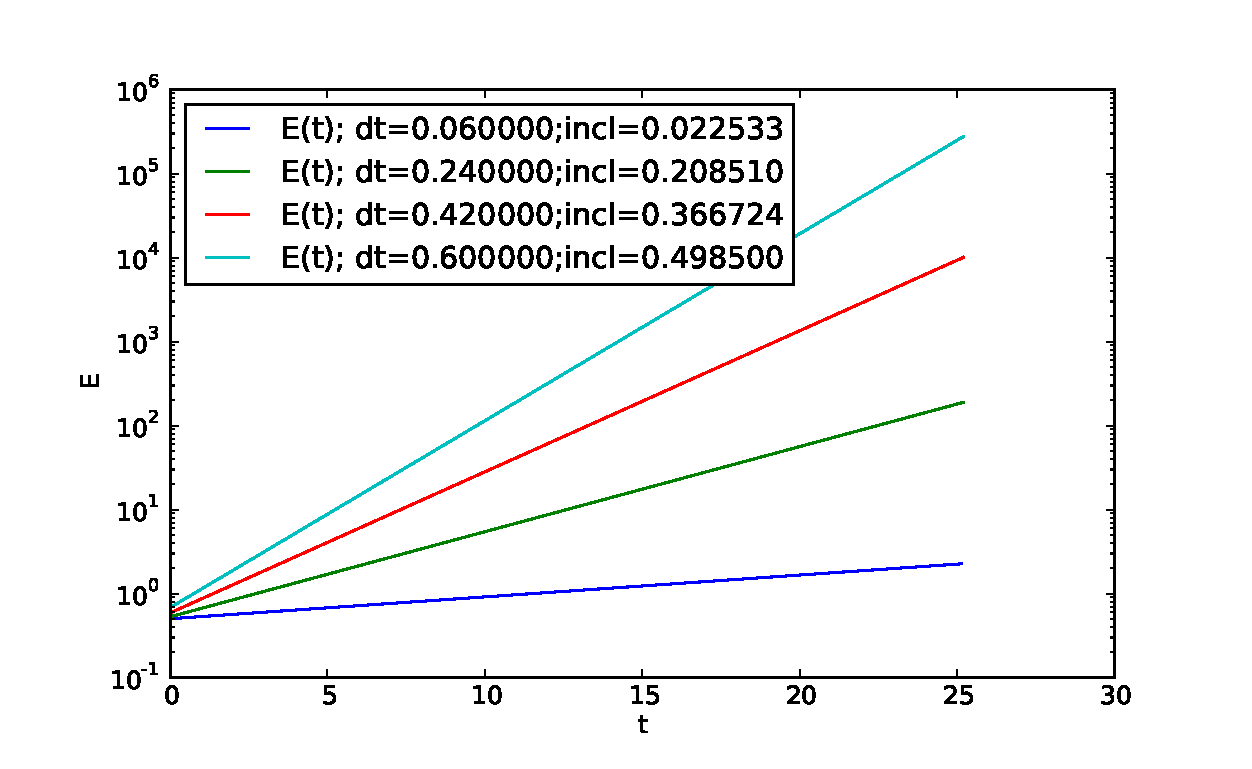
\includegraphics[scale=0.75]{quest3.eps}

\section*{Questão 4} 
As declividades obtidas, listadas no gráfico,
aumentam conforme $\Delta t$ aumenta,
o que significa que quanto maior for $\Delta t$, maior o erro.

A energia aumenta com o tempo porque o erro é acumulado.

\section*{Questão 5} 
$$E(t+\Delta t)=\frac{1}{2}(kx(t+\Delta t)^2+mv(t+\Delta t)^2)$$
$$=\frac{1}{2}(k[x(t)+v(t)\Delta t]^2+m[v(t)-\frac{k}{m}x(t)\Delta t)]^2)$$
$$=\frac{1}{2}(kx(t)^2+2kx(t)v(t)\Delta t+k[v(t)\Delta t]^2+mv(t)^2-2kx(t)v(t)\Delta t+\frac{k^2}{m}[x(t)\Delta t]^2)$$
$$=E(t)+\frac{1}{2}(k[v(t)\Delta t]^2+\frac{k^2}{m}[x(t)\Delta t]^2)$$

\section*{Questão 6} 
Com o algoritmo de Euler-cromer, o erro foi muito pequeno:

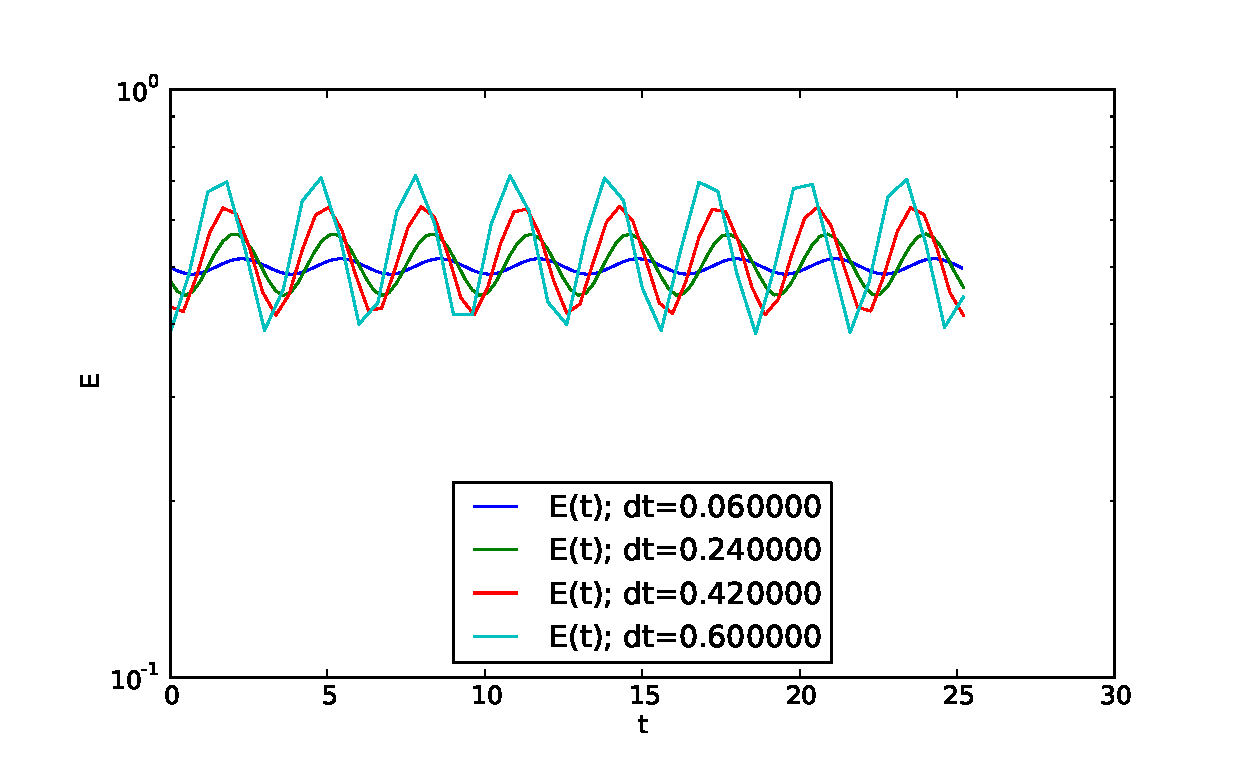
\includegraphics[scale=0.75]{quest6.eps}

Como o erro do valor da energia oscila, ele não é acumulado, 
por isso não aumenta com o tempo.

Valores menores de $\Delta t$ apresentaram oscilações menores.

\section*{Questão 7} 
$k=1$, $m=1$, $\tau=2\pi$

Com Euler e $\Delta t = 0.06s$, a energia duplica 
aproximamente a cada dois períodos.

Com Euler-Cromer e $\Delta t = 0.06s$, a flutuação é próxima de 1 por cento.
\end{document}

